\scanpage{13}
\[
v_p\left(\frac{\pi^n}{n!}\right)\ge0\quad\inserted{\text{\unsure{resp. }} >0}\qquad\text{pour \unsure{tout} }n\ ?
\]
\[
v_p\left(\frac{\pi^n}{n!}\right)\longrightarrow+\infty\qquad\text{pour }n\longrightarrow+\infty
\]
\[
\deleted{\unsure{(p-1)}}\quad v_p\left(\frac{\pi^n}{n!}\right)=\deleted{\unsure{(p-1)}}n v_p(\pi)-\frac{\{n-\operatorname{chif}(n)\}}{p-1}\ge0
\]
\[
\Updownarrow\qquad v_p(\pi)\ge\frac{1-\dfrac{\operatorname{chif}(n)}{n}}{p-1}
\]
\[
\deleted{v_p(\pi)}\qquad\operatorname{chif}(n)/n\longrightarrow0
\]
\deleted{$\dfrac{\operatorname{chif}(n)}{n}$ \unsure{fonction décroissante de $n$, tjs $\le1$}}
\[
\operatorname{chif}(n)\le1
\]
\[\unsure{c}\]
\margin{$\unsure{\frac q6|\ne}$}
\[
\begin{aligned}
n&=a_0+a_1p+\cdots+a_\nu p^\nu\\
\operatorname{chiff}(n)&=a_0+a_1+\cdots+a_\nu
\end{aligned}
\]
si $a_\nu\ne0$, on \unsure{trouve|a}
\[
\begin{aligned}
\operatorname{chiff}n&\le(p-1)\nu\deleted{\unsure{+1}}\\
n&\ge p^\nu\\
\frac{\operatorname{chiff}n}{n}&\le\frac{(p-1)\nu}{p^\nu}\longrightarrow0
\end{aligned}
\]
donc
\figure{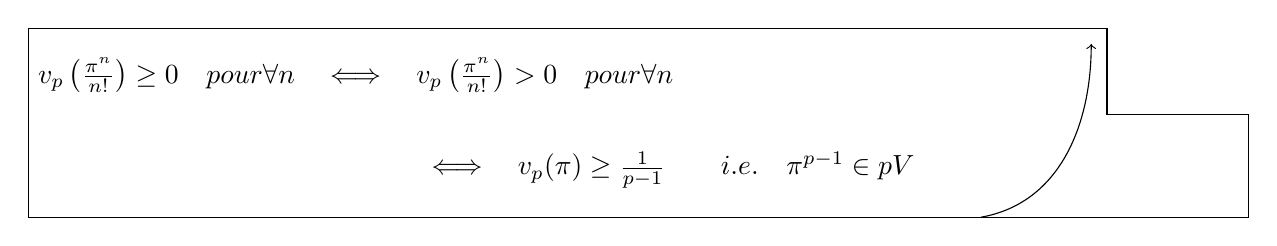
\begin{tikzpicture}
\node[anchor=west] at (0,1.2) {$v_p\left(\frac{\pi^n}{n!}\right)\ge0\quad\text{pour }\forall n\quad\Longleftrightarrow\quad v_p\left(\frac{\pi^n}{n!}\right)>0\quad\text{pour }\forall n$};
\node[anchor=west] at (5,0) {$\Longleftrightarrow\quad v_p(\pi)\ge\frac1{p-1}\qquad\text{i.e.}\quad\pi^{p-1}\in pV$};
\draw (0,1.8)--(13.7,1.8)--(13.7,0.7)--(15.5,0.7)--(15.5,-0.6)--(0,-0.6)--cycle;
\draw[->] (12.1,-0.6) to[out=10,in=-90] (13.5,1.6);
\end{tikzpicture}}
\[
(p-1)v_p\left(\frac{\pi^n}{n!}\right)=n[(p-1)v_p(\pi)-1]+\operatorname{chif}(n)
\]
Si $v_p(\pi)=\dfrac1{p-1}$, c'est $\operatorname{chif}(n)$, qui ne tend pas vers $+\infty$

Si $v_p(\pi)>\dfrac1{p-1}$, on \unsure{trouve} $\underbrace{\alpha n+\operatorname{chif}(n)}_{\displaystyle =n\left(\alpha+\frac{\operatorname{chif}(n)}n\right)\sim\alpha n}$, \inserted{$\alpha>0$,} (qui tend vers $\infty$

Donc \deleted{\unsure{condition}}
\[
\boxed{v_p\left(\frac{\pi^n}{n!}\right)\longrightarrow+\infty\quad\Longleftrightarrow\quad v_p(\pi)>\frac1{p-1}}
\qquad\boxed{\begin{gathered}\text{i.e. }p=\operatorname{unit}\pi^r,\\\text{avec }r<p-1\end{gathered}}
\]
\mspage{12}
